This work provides a novel approach to solve this open problem, and juxtaposes this approach and its experimental results against the current state-of-the-art models. We empirically demonstrate the separation of content and style spaces by demonstrating the inferred spaces of labeled sentences in a sentiment-transfer task, where the positive sentences in the test set are converted to equivalent sentences with a negative sentiment, and vice-versa. We open-source our implementation under a permissive license so that the general framework can be applied to a multitude of other problems that are thematically similar, and rely on modifications of latent attributes in text\footnote{https://github.com/vineetjohn/linguistic-style-transfer}.

In this section, we describe our approach in detail. Our model is built upon an autoencoder with a sequence-to-sequence (Seq2Seq) neural network~\cite{sutskever2014sequence}, as described in Subsection~\ref{ss:seq2seq}. Then we introduce two auxiliary losses, multi-task loss and adversarial loss in Subsections~\ref{ss:multi} and \ref{ss:adv}, respectively. Subsection~\ref{ss:prediction} presents the approach to transfer style in natural language generation. Figure~\ref{fig:model-overview} depicts both training and prediction processes of our approach.

\begin{figure}[ht]
	\centering
	\includegraphics[width=0.9\linewidth]{images/model-overview.png}
	\caption{Overview of our approach.}
	\label{fig:model-overview}
\end{figure}

\subsection{Autoencoder}\label{ss:seq2seq}

An autoencoder encodes an input to a latent vector space, from which it decodes the input itself. By doing so, the autoencoder learns meaningful representations of data. This serves as our primary learning objective. Besides, we also use the autoencoder for text generation in the style-transfer application.

Let $\rmx=(x_1, x_2, \cdots x_n)$ be an input sentence. The encoder encodes $\rm x$ by a recurrent neural network (RNN) with gated recurrent units (GRU) \cite{cho2014learning}, and obtains a hidden state $\bm h$.

Then a decoder RNN generates a sentence, which ideally should be $\rmx$ itself. Suppose at a time step $t$, the decoder RNN predicts the word $x_t$ with probability $p(x_t|\bm h, x_1\cdots x_{t-1})$, then the autoencoder is trained with cross-entropy loss, given by
\begin{equation}\nonumber
	J_\text{rec}(\bm\theta_E,\bm\theta_D)= -\sum_{t=1}^n \log
	p(x_t|\bm h, x_1\cdots x_{t-1})
\end{equation}
where $\bm\theta_E$ and $\bm\theta_D$ are the parameters of the encoder and decoder, respectively.

Since this loss trains the autoencoder to reconstruct $\rmx$, it is also called \textit{reconstruction loss}.

Besides the above reconstruction loss, we design two auxiliary losses to disentangle the latent space $\bm h$. In particular, we hope that $\bm h$ can be separated into two spaces $\bm s$ and $\bm c$, representing style and content respectively, i.e., $\bm h = [\bm s ; \bm c]$, where $[\cdot;\cdot]$ denotes concatenation. This is accomplished by the below auxiliary losses.

\subsection{Multi-Task Loss} \label{ss:multi}

Our first auxiliary loss ensures the style space does contain style information. We build a classifier on the style space $\bm s$ predicting the style label $s$, which is a part of the training data.

This loss can be viewed as a \textit{multi-task} loss, which makes the neural network not only decode the sentence, but also predicts its sentiment. Similar multi-task losses are used in previous work for sequence-to-sequence learning \cite{luong2015multi}, sentence representation learning \cite{jernite2017discourse} and sentiment analysis \cite{balikas2017multitask}, among others.

In our application, we follow previous work \cite{hu2017toward,shen2017style,fu2017style} and treat the sentiment as the style of interest. We introduce a binary classifier
\begin{equation}
	p(s=1|\bm s;\bm\theta_\text{mult})=\sigma(\bm w_\text{mult}^\top \bm s + b_\text{mult})
\end{equation}
where $\bm\theta_\text{mult}=[\bm w_\text{mult}; b_\text{mult}]$ are the classifier's parameters for multi-task learning.
\begin{align} \label{eqn:Jmult}
	 & J_\text{mult}(\bm\theta_{E};\bm\theta_\text{mult})=                \\ \nonumber
	 & -s\log p_\text{mult}(s|\bm s) - (1-s)\log p_\text{mult}(1-s|\bm s)
\end{align}
where $\bm\theta_E$ are the encoder's parameters. (Notice that the bold letter $\bm s$ represents the encoded style vector, whereas the unbold letter $s$ represents the binary style label).


\subsection{Adversarial Learning} \label{ss:adv}

The above multi-task loss only operates on the style space, but does not have an effect on the content space $\bm c$.

We therefore apply an adversarial loss to disentangle the content space from style information, inspired by adversarial generation~\cite{goodfellow2014generative}, adversarial domain adaptation~\cite{liu2017adversarial}, and adversarial style transfer~\cite{fu2017style}.

The idea of adversarial loss is to introduce an adversary that deliberately discriminates style $s$ on the content vector $\bm c$. Then the autoencoder is trained to learn such a content vector space that its adversary cannot predict style information.

Concretely, the adversarial discriminator predicts style $s$ by a logistic regression
\begin{equation}
	p_\text{dis}(s=1|\bm c;\bm\theta_\text{adv})=\sigma(\bm w_\text{adv}^\top \bm c + b_\text{adv})
\end{equation}
where $\bm\theta_\text{dis}=[\bm w_\text{dis}; b_\text{dis}]$ are the parameters of the adversary. It is trained by
\begin{align}
	 & J_\text{dis}(\bm\theta_\text{dis})=                            \\ \nonumber
	 & -s\log p_\text{dis}(s|\bm c)-(1-s)\log p_\text{dis}(1-s|\bm c)
\end{align}
The adversarial loss appears similar to the multi-task loss as in Eq.~(\ref{eqn:Jmult}). However, it should be emphasized that, for the adversary, the gradient is not propagated back to the autoencoder, i.e., $\bm c$ is treated as shallow features.

Having trained an adversary, we would like the autoencoder to be tuned in such an \textit{ad hoc} fashion, that $\bm c$ is not discriminative in style. In other words, we penalize the entropy of the adversary's prediction, given by
\begin{equation}
	J_\text{adv}(\bm\theta_E)=\mathcal{H}(p_\text{dis}(s|\bm c))
\end{equation}
where $\mathcal{H}=-\sum_{i\in\text{labels}}p_i\log p_i$ is the entropy. The adversarial objective is maximized, in this phase, with respect to the encoder.



\subsection{Training Process}

To put it all together, our training process is a loop of the following processes:
\begin{itemize}
	\item minimize $J_\text{dis}(\bm\theta_\text{dis})$ w.r.t. $\bm\theta_\text{dis}$, and
	\item minimize $J_\text{rec}(\bm\theta_E, \bm\theta_D) + \lambda_\text{mult}(\bm\theta_E,\bm\theta_\text{mult}) -\lambda_\text{adv}
		      J_\text{adv}(\theta_E)$ w.r.t. $\bm\theta_E, \bm\theta_D, \bm\theta_\text{mult}$.
\end{itemize}
where $\lambda_\text{mult}$ and $\lambda_\text{adv}$ balance these losses.

We use the Adam optimizer \cite{kingma2014adam} with an initial learning rate of $10^{-3}$ and train the model for 50 epochs. Both the autoencoder and its adversary are trained once per epoch with $\lambda_\text{mult} = 1$ and $\lambda_\text{adv} = 0.3$.

\subsection{Generating Style-Transferred Sentences} \label{ss:prediction}

A direct application of our disentangled latent space is style transfer for natural language generation. For example, we can generate a sentence with generally the same meaning (content) but an opposite sentiment.

Let $\rmx_*$ be an input sentence with $\bm s_*$ and $\bm c_*$ being the encoded, disentangled style and content vectors, respectively. If we would like to transfer its content to a different style, we compute an empirical estimate of the target style's vector $\hat{\bm s}$ by
$\hat{\bm s}=\frac{\sum_{i\in\text{target style}}\bm s_i}{\text{\# target style samples}}$. The inferred target style $\hat{\bm s}$ is concatenated with the encoded content $\bm c_*$ for decoding (Figure~\ref{fig:model-overview}b).

\section{Experiments}
We conducted experiments on an Amazon product review dataset, following \cite{fu2017style}. It contains 131072, 2048, 32768 sentences for train, validation, and test, respectively, each sampling accompanied by binary sentiment labels.

\subsection{Disentangling Latent Space}


We first analyze how the style (sentiment) and content of the latent space are disentangled. We train a logistic classifier based on different latent spaces, and show results in Table~\ref{tab:classification}.

We see that the 128-dimensional content vector is not discriminative for style. It achieves an accuracy of 57\%, slightly better than random/majority guess. However, the 8-dimensional style vector $\bm s$, despite its low dimensionality, achieves significantly higher style classification accuracy. When combining content and style vectors, we achieve no further improvement. These results verify the effectiveness of our disentangling approach, because the style space does contain style information, whereas the content space doesn't.


\begin{table}
	\centering
	\begin{tabular}{| l | r |}
		\hline
		Random/Majority guess           & 0.5000          \\ \hline
		Content latent space  ($\bm c$) & 0.5690          \\
		Style latent space ($\bm s$)    & \textbf{0.7817} \\
		Combined ($[\bm s;\bm c]$)      & 0.7815          \\
		\hline
	\end{tabular}
	\caption{Style classification accuracy.}
	\label{tab:classification}
\end{table}

\begin{figure}
	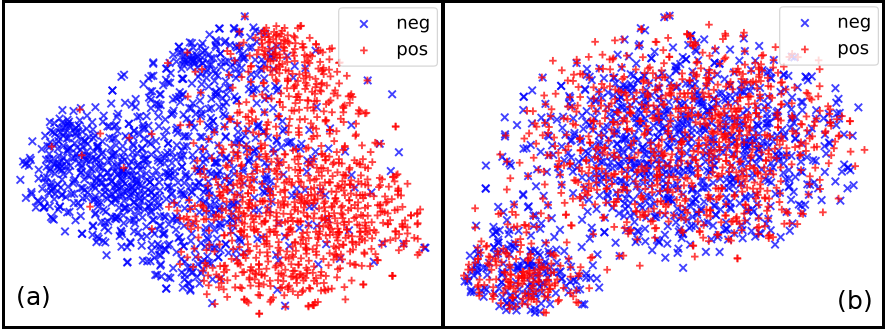
\includegraphics[width=\linewidth]{images/tsne-style-and-content}
	\caption{t-SNE plots of (a) style and (b) content spaces.}
	\label{fig:tsne}
\end{figure}


The latent space can be visualized with t-SNE plots~\cite{maaten2008visualizing} in Figure~\ref{fig:tsne}. As expected, sentences with different sentiments can be nicely separated in the style space (LHS), but are highly mixed in the content space (RHS).


\subsection{Style-Transfer Sentence Generation}

We apply the disentangled latent space to a style-transfer sentence generation task, where the goal is to generate a sentence with different sentiment (style). We followed \cite{fu2017style} and used two metrics: (1) For style transfer, we train a style classifier and predict the accuracy of the generated sentences. While the style classifier itself may not be perfect, it provides a quantitative way of evaluating the strength of style transfer. (2) For the content-preservation score, we compute a sentence embedding by min, max, and average pooling of word embeddings; then a cosine similarity is computed to evaluate how close two sentences are in meaning. Here, sentiment words from a stop list \cite{hu2004mining} are removed.

We compare our approach with state-of-the-art previous work in Table~\ref{tab:comparison-previous}. We re-conducted the experiments with their publicly available code on our data splits.
Results show that, our approach achieves a comparable content-preservation score with previous work, but a significantly better style-transfer score, showing that our disentangled latent space can be used for better style-transfer sentence generation.

Table~\ref{tab:ablation-results} presents the results of an ablation test. We see that both adversarial loss and reconstruction loss play a role in the strength of style transfer, and that they can be combined to further improve performance.

Some examples of style-transfer sentence generation are illustrated in Table~\ref{tab:transfer-samples}. We see that, with the empirically estimated style vector, we can flexibly control the sentiment of generated sentences.

\begin{table}[!t]
	\centering
	\begin{tabular}{| l | r | r | }
		\hline
		\textbf{Model}                       & \textbf{Style Transfer} & \textbf{Content Preservation} \\
		\hline
		\hline
		Cross-alignment \cite{shen2017style} & 0.4609                  & 0.8830                        \\
		\hline
		Sentiment embed. \cite{fu2017style}  & 0.4009                  & 0.9246                        \\
		\hline
		Ours                                 & 0.7708                  & 0.8958                        \\
		\hline
	\end{tabular}
	\caption{Comparison with previous approaches.}
	\label{tab:comparison-previous}
\end{table}

\begin{table}[!t]
	\centering
	\begin{tabular}{| l | r | r |}
		\hline
		\textbf{Training Loss}                          & \textbf{Style Transfer} & \textbf{Content Preservation} \\
		\hline
		\hline
		$J_\text{rec}$                                  & 0.5053                  & 0.9103                        \\
		\hline
		$J_\text{rec}$, $J_\text{adv}$                  & 0.5901                  & 0.9121                        \\
		\hline
		$J_\text{rec}$, $J_\text{mult}$                 & 0.6445                  & 0.9053                        \\
		\hline
		$J_\text{rec}$, $J_\text{adv}$, $J_\text{mult}$ & 0.7708                  & 0.8958                        \\
		\hline
	\end{tabular}
	\caption{Ablation test.}
	\label{tab:ablation-results}
\end{table}

\begin{table}[!t]
	\centering
	\begin{tabular}{| p{0.45\linewidth} | p{0.45\linewidth} |}
		\hline
		\textbf{{Original}}                                                        & \textbf{Transferred (Positive $\rightarrow$ Negative)}                    \\
		\hline
		\hline
		i bought this cuisipro mister to replace my old mister last june-(number)  & i bought this a couple of times and was disappointed in this product      \\
		\hline
		quality is good, recevied in time and works as expected.                   & quality is good but i am returning it                                     \\
		\hline
		all in all, i am very happy with this headset.                             & all in all i was expecting a good product                                 \\
		\hline
		\hline
		\textbf{{Original}}                                                        & \textbf{Transferred (Negative $\rightarrow$ Positive)}                    \\
		\hline
		\hline
		i sent it back and requested a refund, and never got the refund.           & i sent it back and gave it a try and it works great                       \\
		\hline
		so i tried just one (number) piece each n still the same results.          & so i bought the two sizes and the other ones are great                    \\
		\hline
		i am going to buy a replacement and wish i had sent this back for a refund & i am going to go through the same time and i have been using it for years \\
		\hline
	\end{tabular}
	\caption{Examples of style-transfer generation.}
	\label{tab:transfer-samples}
\end{table}
